

%TODO
%	Different scheduling types on the for loop
% 	
\documentclass[10pt,letterpaper]{article}

\usepackage{cvpr}
\usepackage{times}
\usepackage{epsfig}
\usepackage{graphicx}
\usepackage{amsmath}
\usepackage{amssymb}
\usepackage{algorithm}
\usepackage{algorithmic}
\usepackage{etoolbox}\AtBeginEnvironment{algorithmic}{\footnotesize}
\usepackage{graphicx}
\usepackage{subcaption}

\usepackage{abstract}
\renewcommand{\abstractname}{Introductory Note on the System}    % clear the title

% Include other packages here, before hyperref.

% If you comment hyperref and then uncomment it, you should delete
% egpaper.aux before re-running latex.  (Or just hit 'q' on the first latex
% run, let it finish, and you should be clear).
\usepackage[breaklinks=true,bookmarks=false]{hyperref}

\cvprfinalcopy % *** Uncomment this line for the final submission

\def\cvprPaperID{****} % *** Enter the CVPR Paper ID here
\def\httilde{\mbox{\tt\raisebox{-.5ex}{\symbol{126}}}}

% Pages are numbered in submission mode, and unnumbered in camera-ready
%\ifcvprfinal\pagestyle{empty}\fi
\setcounter{page}{1}
\begin{document}

%%%%%%%%% TITLE
\title{A Parallelized Framework for Evolutionary Computation}

\author{
	Geoffrey Saxton Long (\textit{260403840})\\
	McGill University, Quebec \\
	{\tt\small Geoffrey.Long@mail.mcgill.ca}
}

\maketitle
%\thispagestyle{empty}

%%%%%%%%% ABSTRACT
\begin{abstract}
The file \texttt{parallel\_GA.cpp} can be compiled via \texttt{g++ -fopenmp parallel\_GA.cpp}. It the program fails to compile see \texttt{NOTE1} in the code, implement the changes, and recompile. It can then be run by via the command line with \texttt{./a.out}. If you would like to try out a different version they are tagged on github. These versions, and all the other files, can be found on \url{https://github.com/GeoffreyLong/Parallelized_GA}.

The discussions cover only a subset of the testing and material conducted for the project. More testing instances can be found on Github under the \texttt{Results} subfolder. In (almost) all of the files, the columns are as follows: number of threads, population size, number of iterations, fitness, speedup, (runtime). Though the vast majority of the files follow this format, several of the earlier tests could have slightly different configurations. All of these instances were averaged over at least five runs, and most of them are averaged over ten runs. In addition to the testing instances, the matlab programs for graphing can be found there as well as as the initial attempt at a distributed genetic algorithm framework. The plan for the distributed framework was to run it similar to the parallel program, but to have each rank take on a different series of evolutionary operators. From this, I expected to have divergent behaviour on each host, a more varied set of populations, and therefore higher chances of finding an optimal solution.
\end{abstract}

% http://watchmaker.uncommons.org/manual/ch01s02.html
% EC is good for problems where you know what comprises a good solution, but you don't necessarily know how to reach this solution.

\newpage
\section{Introduction}
Evolutionary Computation is a branch of computational intelligence commonly used to solve problems with complex relationships between the parameters, multiple local optima, or no known approach. The term \textit{evolutionary computation} covers several different algorithmic approaches. The four main ones are evolutionary programming, genetic programming, genetic algorithms, and evolution strategies \cite{ecomp}. Although each of these frameworks is slightly different, they all have the same general structure and themes; specifically, the adherence to Darwinian principles.

The darwinian principles central to evolutionary computation are those of evolution by natural selection. This is commonly broken into four main themes \cite{naturalselection,naturalselection2}:
\begin{enumerate}
\item More individuals are produced each generation than can survive
\item Variation exists among individuals, this variation is inheritable
\item Those individuals with inherited traits better suited to the environment will survive
\item When reproductive isolation occurs a new species will form
\end{enumerate}

The above can be abstracted easily into programming. To model evolution in a computer environment you need encodings for a set of individuals, and operators to create variety within the individuals. Central to evolutionary computation is the \textit{population}. This population is a set of \textit{individuals}, which are each an encoding of a possible solution. The individuals can be analyzed on how well they solve the underlying problem. This analysis is called \textit{fitness evaluation} and the score attributed to each individual is called its \textit{fitness}.

Commonly these individuals are bit strings, however they can have more complex structures. The way in which the individual is encoded is often unique to the problem and specific implementation. The individual can be optimized to be space efficient, easily manipulated, or easily understood. The encoding will only be successful if it can be altered by the evolutionary operators in the framework.

The evolutionary operators most commonly used are \textit{mutation} and \textit{crossover}. Although mutation is present in all evolutionary computation methods, crossover is often specific to certain subsets of evolutionary computation such as genetic algorithms. Both of these operators act on \textit{alleles}, which are the smallest differentiable part of each individual. % Differentiable isn't really the right word, more like the smallest unit that can stand alone, or the smallest that can have a healthy abstraction

Mutation is the alteration of an individual via a slight change in their genetic makeup. This change typically occurs through changing the value one of the individual's alleles or by switching two or more alleles. The resultant individual is slightly different from the original. The implementation determines how slight this difference is.

Crossover involves the creation of a new individual by combining two or more "parent" individuals. Typically, the parents are selected based on their genetic fitness; the fittest individuals are usually allowed to procreate. When the parents are selected, the crossover operators usually use sections of each to create one or more new individuals. These operators involve combining snippets from each parent to create the individual.

The individuals in a population are operated on iteratively. Each iteration is called a \textit{generation}, and typically involves both mutations and crossovers. Since the population at the end of each iteration is larger than the previous, the final step in the iteration is to "kill" off certain individuals. This is known as \textit{selection}, and holds closest to the themes of natural selection. The goal of each iteration is to stochastically approach an optimal fitness value. The program will iterate over generations until it reaches a termination criteria, which is commonly based on a number of iterations or on some fitness metric. Upon termination, the top performing individual are returned as the solution to the problem.


\section{Background}
% Previous algorithms, previous attempts at parallelization?
In order to test the framework, I chose to implement the travelling salesperson algorithm. In this algorithm you are given an undirected fully connected graph. The edges are each weighted, the weights correspond to the cost of traversing the edge. The goal is to find the least cost cycle that reaches each node at least once.

The travelling salesperson problem (TSP) is an NP-hard problem. As such, not only are we unable to compute the optimal solution in polynomial time, an optimal solution cannot even be verified in polynomial time. The TSP has many applications such as routing shipments and manufacturing goods \cite{tspuses}. Due to the importance of these applications, the TSP has become one of the most studied problems in computer science.

There are many different ways to approach TSP. There are exact methods such as simplex programming and linear programming methods, however, these suffer from prohibitively long execution times. More commonly, approaches to the TSP are often approximation algorithms. These give reasonable results within a reasonable execution time. These include optimization, nearest neighbor searching, heuristical approaches, and, of course, evolutionary approaches \cite{matai2010traveling}.


\section{Implementation} \label{sec:implementation}
The remainder of the paper covers the implementation of a parallelized evolutionary framework. All of the tests were conducted using data from TSPLib \cite{tsplib}, specifically the symmetric datasets. All the tests were conducted using one of two machines:
\begin{enumerate}
\item Lenovo: A Lenovo ideapad with an Intel(R) Core(TM) i5-4200U CPU @ 1.60GHz. This processor has two cores with two threads per core. With hyperthreading this creates four virtual cores.
\item Debondt: A McGill CIM server equipped with two Intel(R) Xeon(R) E5645 @ 2.40GHz processors. Each of these have 6 cores (12 with hyperthreading). This results in 12 actual and 24 virtual cores overall.
\end{enumerate}

\subsection{Primary version (v1.1)}
The first iteration of the evolutionary framework was a simple mutation and fitness-based selection algorithm. Essentially, it consisted of two loops. The outer loop counts the generation number and is responsible for terminating the program after a specific number of iterations. The inner loop is a for loop over all the individuals in the population. In this loop, the individual is first mutated via a swap (two cities are selected at random and switched). The mutation returns a new individual, which is compared to the previous (nonmutated) parent. The fitter of the two is selected for the next generation. No crossover was implemented in this version. Since this was the case, this implementation was more of an evolutionary programming method.

Parallelization could not occur over the encapsulating iteration loop as the input of the loop depends on the output of the previous iteration. This linearity in generations is crucial to the evolution. The population loop, on the other hand, was parallelizable because the individuals in the population were independent from one another. So an openmp for loop was placed around the population loop.

The purpose of this version was to characterize the relationships between the various parameters. The parameters compared in this phase were the number of threads, the population size, and the number of iterations. They were evaluated as per their impact on fitness and execution time. The goal was to find relationships between these parameters. By finding relationships, further testing could be constrained by focusing on only the most important parameters.


\subsubsection{Parameter Relationships}
The first tests focused on analyzing how fitness varied with the parameters. The first parameter of interest was the number of threads. Since the number of threads does not change the underlying computations, the fitness should be unaffected by an increase in the thread count. By manual inspection of the data, this was shown to be true. Since these two are uncorrelated, the fitness score of individuals can be largely left out when discussing the efficacy of the parallel implementation. While characterizing fitness versus thread count, it was also found that while an increase in population size does improve the fitness of the individual, there is a larger increase in fitness when the number of iterations is bolstered.

Since fitness proved to be rather irrelevant in the discussion of the parallel performance, speedup and runtime were focused on next. An almost linear relationship was found between the impact of population size on execution time the impact of iteration count on execution time. Doubling either the maximum number of iterations or the population size almost doubles the execution time. Therefore, population size and number of iterations seem to be directly proportional in their effect on execution time

Since we can take the population size and number of iterations to be roughly equal in their impact on execution time, we can easily compare the two under different thread counts. This comparison involved graphical analysis of the relative execution times. In this, population size and number of iterations were varied independently over a range of thread counts. From the graph in Figure \ref{fig:itervspop}, it can be seen that the number of threads impact both the same. So, when the number of iterations and the population size are both much greater than the number of threads, a change in the population size or the number of iterations will have generally the same effect on speedup.

\begin{figure}
\centering
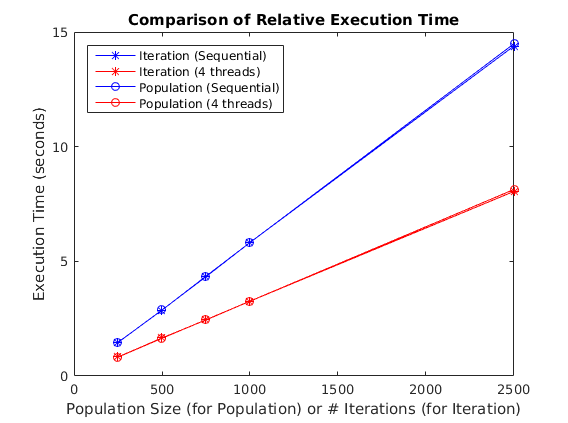
\includegraphics[width=0.6\textwidth]{../img/Lenovo_Compare_ItervsPop.png}
\caption{The effect of different thread counts and population/iteration sizes on runtime.}
\label{fig:itervspop}
\end{figure}

\newpage

This relationship only holds for small thread counts though. As the number of threads approaches the population size, the speedup decreases quickly. This is shown by the graphs of population size vs thread count (Figure \ref{fig:popvsthreads}). Although this relationship exists between population size and speedup, there doesn't appear to be any relationship between number of iterations, number of threads, and speedup. This is shown by the graphs in Figure \ref{fig:itervsthreads}. The reason why the population size has such a large effect is due to how the algorithm is parallelized. The OpenMP parallel construct was placed around a loop over the individuals in a population. When the number of threads increases, each thread is responsible for fewer and fewer individuals. When the number of threads is equal to the population size, each thread is responsible for one loop over one individual. The cost of spawning a thread is great when compared to the relatively small amount of work the thread is responsible for. As an aside, an anomaly worth noting is that for 24 threads the Debondt system has no speedup at all. This is further discussed in Section \ref{sec:discussion}.


\begin{figure}[t]
\centering
  \begin{subfigure}{0.49\linewidth} \centering
	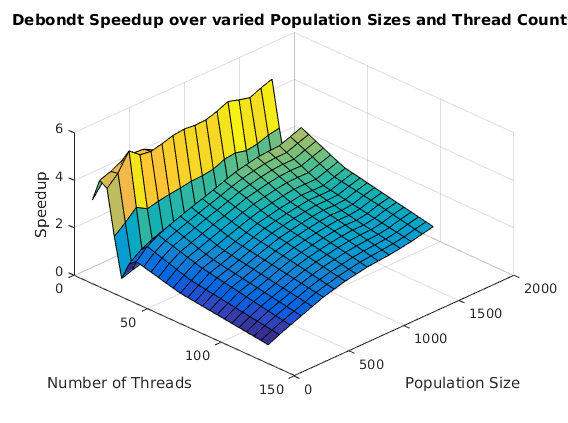
\includegraphics[width=\textwidth]{../img/Debondt_PopulationvsThreads.png}
    \caption{Debondt}\label{fig:figA}
  \end{subfigure}
  \begin{subfigure}{0.49\linewidth} \centering
	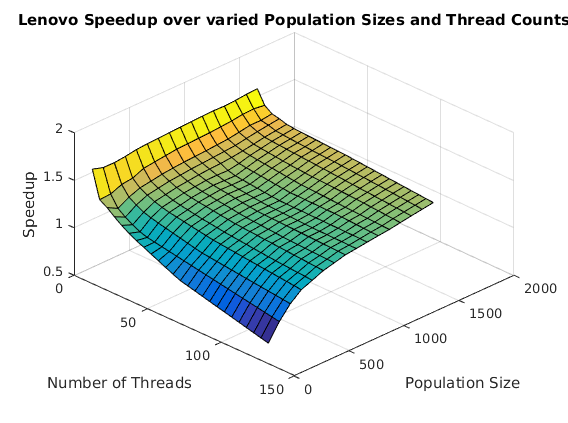
\includegraphics[width=\textwidth]{../img/Lenovo_PopulationvsThreads.png}        
    \caption{Lenovo}\label{fig:figB}
  \end{subfigure}
\caption{ffect of population size and number of threads on speedup (EIL51).} \label{fig:popvsthreads}
\end{figure}


\begin{figure}[t]
\centering
  \begin{subfigure}{0.49\linewidth} \centering
	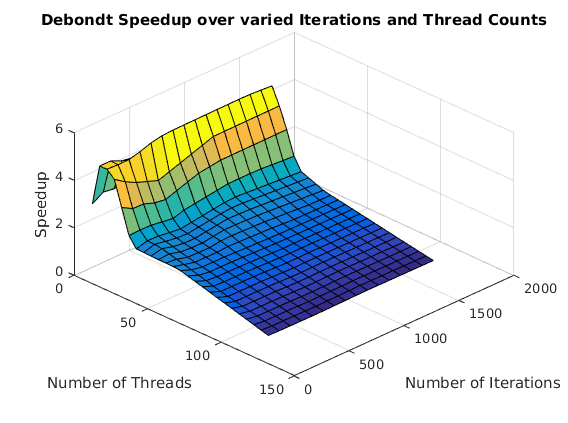
\includegraphics[width=\textwidth]{../img/Debondt_IterationvsThreads.png}
    \caption{Debondt}\label{fig:figA}
  \end{subfigure}
  \begin{subfigure}{0.49\linewidth} \centering
	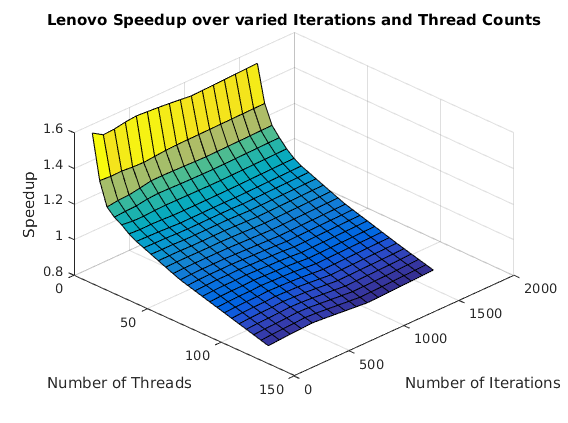
\includegraphics[width=\textwidth]{../img/Lenovo_IterationvsThreads.png}
    \caption{Lenovo}\label{fig:figB}
  \end{subfigure}
\caption{Effect of number of iterations and number of threads on speedup (EIL51).} \label{fig:itervsthreads}
\end{figure}

\newpage
So, based on the above, if the population size is sufficiently high, the population size and iteration count can essentially be left out of conversations on speedup. In order to accurately calculate speedup, an ideal number for population size and maximum number of iterations was ascertained. This was found by running the program on the Lenovo with a set number of threads and a varying population size and iteration number. From the resultant graph (Figure
\ref{fig:popvsiter}), I found that a population size of 250 with an iteration number of 10000 was ideal for further testing on the Lenovo machine. On Debondt, the ideal population size seemed to be closer to 500 individuals. These parameter values maximized the speedup and minimized the overall execution time while still providing a good final fitness. The aforementioned sizes were run on Debondt and Lenovo with variable thread counts to characterize the speedup. From these trials I got the graphs in Figure \ref{fig:EILspeedups}.


\begin{figure}
\centering
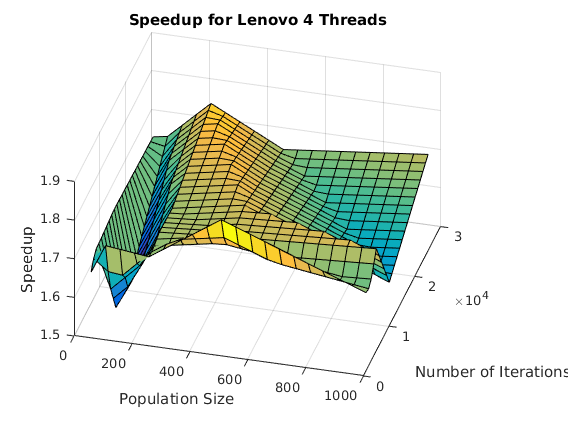
\includegraphics[width=0.6\textwidth]{../img/Lenovo_4Thread_PopvsIter.png}
\caption{Impact of population size and number of iterations on overall speedup (Lenovo - 4 threads - EIL51).}
\label{fig:popvsiter}
\end{figure}



\begin{figure}[t]
\centering
  \begin{subfigure}{0.49\linewidth} \centering
	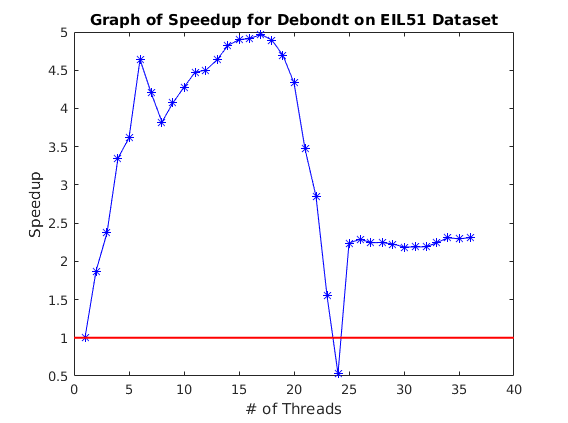
\includegraphics[width=\textwidth]{../img/Debondt_speedup.png}
    \caption{Speedup of Debondt over the EIL51 dataset.}\label{fig:figA}
  \end{subfigure}
  \begin{subfigure}{0.49\linewidth} \centering
	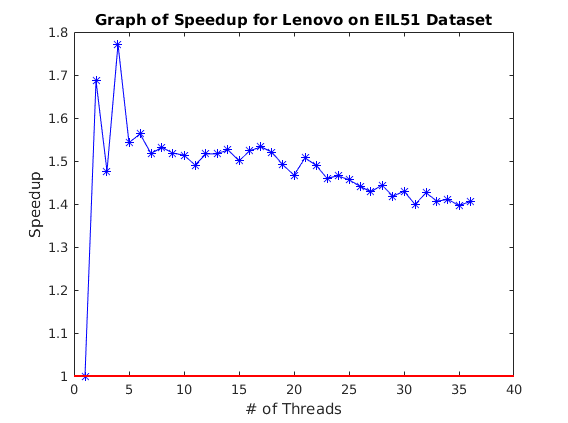
\includegraphics[width=\textwidth]{../img/Lenovo_Speedup.png}
    \caption{Speedup of Lenovo over the EIL51 dataset.}\label{fig:figB}
  \end{subfigure}
\caption{Speedups of Debondt and Lenovo (EIL51 - v1.1} \label{fig:EILspeedups}
\end{figure}


The final trials run on version v1.1 involved determining the effects of tour size on the speedup. Thankfully, I had a few different tours of varied length. These were run using Debondt and the outcome was graphed in Figure \ref{fig:tours}. As is shown, the larger the tour size, the larger the speedup.

\begin{figure}
\centering
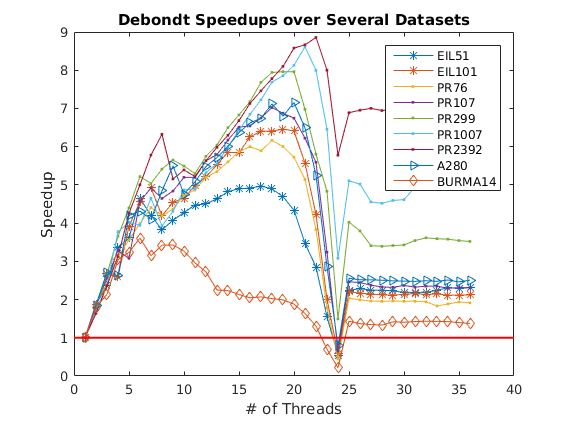
\includegraphics[width=0.6\textwidth]{../img/dataset_speedups.png}
\caption{Impact of tour length on overall speedup (Debondt).}
\label{fig:tours}
\end{figure}

\clearpage
\newpage
\subsection{Two Loop Version (v1.4)}
This version was an optimized version of the initial. The first change was to move the \texttt{openmp parallel} construct to the outside of the first loop. This reduced overhead since threads did not have to be spawned and killed at every generation. The second change was the parallelization of population instantiation. This instantiation takes all the cities and creates individuals by scrambling the ordering, resulting in a random tour. Previously this was omitted from parallelization since the initialization was expected to take little time in comparison to the population loop. The section was parallelized in this version using another pragma for loop. Since the work inside the for loop involved adding an object to a shared vector, a critical section had to be inserted. The critical section encapsulates the pushing of the individual to the population vector.

The bulk of the parallelization still occurs at the inner population loop as before. Several different loop schedules were attempted for the inner loop, however, the default seemed to work the best for the Lenovo system. This schedule, static looping over large chunks, works best because each individual should take roughly the same amount of work. It also has reduced overhead when compared to the more dynamic scheduling systems.


\subsection{Three Loop Version (v1.5)}
This version saw an added parallelization for the fittest individual calculations. This fitness calculation is performed at the end of the iterative process. It finds the the fittest individual in the population. Similar to the initialization loop, this calculation was viewed as trivial in comparison to the main iterative loop. Although the increase in speedup was expected to be rather small, the optimization was still performed. 

Since this loop involves storing the top fitness value in a public object, a critical section needed to be added. Although an atomic operation was deemed to have less overhead \cite{atomicoverhead}, it would not work properly for the encapsulated assignment. The critical section was eventually replaced by a reduction clause, since a reduction seemed to have less overhead in addition to being more dynamic \cite{suss2008common}. The result was a parallelized for loop where each thread gets its own copy of the best fitness value. At the end of the loop openmp will reduce this array of fitness values to find the optimal value.

In addition to the added parallelization, the population initialization was optimized. The critical section in the population parallelization was viewed as unnecessary synchronization. The first option was to remove the critical section by directly accessing the indices on writes. I decided not to proceed with this change because it would involve changing the vector datatype, and it could introduce false sharing along with other unfavorable conditions. Luckily, I found a better alternative. This was to declare an openmp reduction function for merging the vectors created by each individual thread. The resultant vectors from each thread are merged out of order, but this is actually preferred since the individual creation is supposed to be randomized. Optimizing this loop required an update to GCC 4.9 (OpenMP 4.0), but was otherwise rather simple.

Although this worked on the Lenovo, Debondt did not have GCC 4.9. So, "v1.5 critical" was created to test this version on Debondt. Unfortunately, this uses the aforementioned critical section, so there is a decent amount of synchronization occurring. With this version, different schedulings were tested. Contrary to what was believed earlier, static is not the best scheduler for this program. Based on Figure \ref{fig:schedules}, runtime is actually the fastest. Although static works best for the Lenovo, Debondt works best with runtime. Static was actually the poorest performing on Debondt. This could be because of the critical synchronization.


\begin{figure}
\centering
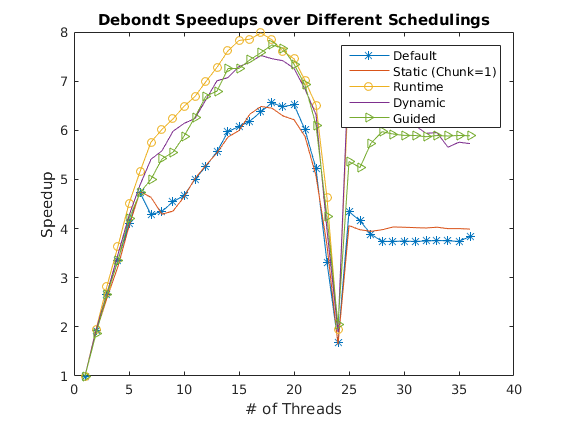
\includegraphics[width=0.6\textwidth]{../img/debondt_schedulers.png}
\caption{Speedup comparison of different loop scheduling constructs (Debondt - EIL51 - v1.5 Critical).}
\label{fig:schedules}
\end{figure}

\subsection{Final Version (v1.6)}
The final optimizations mostly had to do with changing the scheduling for the loops. As was shown before, the schedule that works best is the "runtime" schedule. The schedule was added to only the population loop. This decision was mostly based on the fact that the population loop is the most dynamic due to the mutation methods. Also, the mutation operator was switched as well. Previously most tests were conducted using the swap mutation, however, inversion was shown to have both the best fitness results and the greatest speedup. This can be seen in Figure \ref{fig:mutations}. The final alteration for version v1.6 was preallocating the vectors.

\begin{figure}[t]
\centering
  \begin{subfigure}{0.49\linewidth} \centering
	 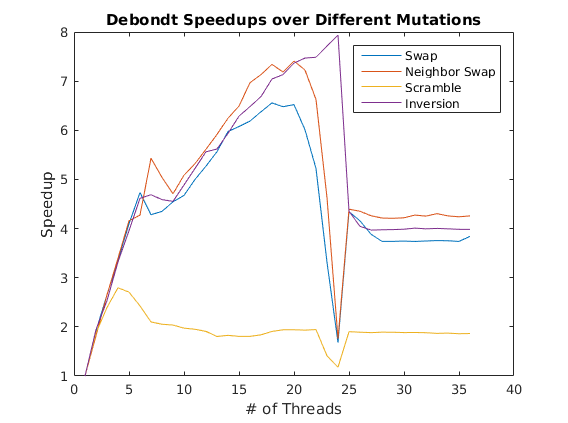
\includegraphics[width=\textwidth]{../img/Debondt_mutations_speedup.png}
    \caption{Speedup}\label{fig:figA}
  \end{subfigure}
  \begin{subfigure}{0.49\linewidth} \centering
	 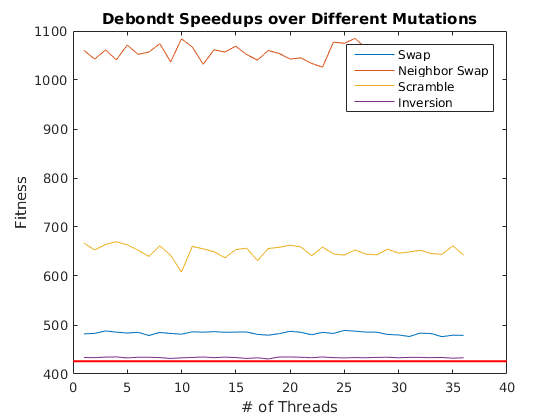
\includegraphics[width=\textwidth]{../img/Debondt_mutations_fitness.png}
    \caption{Fitness (Optimal=426)}\label{fig:figB}
  \end{subfigure}
\caption{Effect of different mutations on Speedup and Fitness (EIL51 - Debondt - v1.5Critical} \label{fig:mutations}
\end{figure}

\newpage
\section{Results} \label{sec:results}
The three versions were tested with the EIL51 dataset with a population size of 500 and an iteration count of 10000. Unfortunately, version v1.5 could not be tested on Debondt due to compiler issues, so v1.5 critical was used instead. The resulting speedups are shown in Figure \ref{fig:versions}. As can be seen, the speedup of v1.4 was faster than v1.5 critical. This was likely due to the synchronization overhead of the critical section in v1.5 critical.

\begin{figure}
\centering
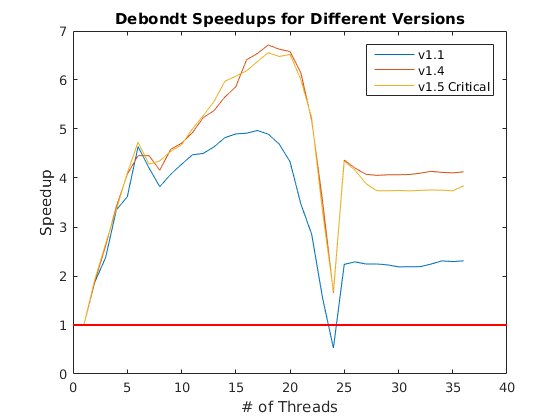
\includegraphics[width=0.6\textwidth]{../img/debondt_versions.png}
\caption{Speedup comparison of versions v1.1, v1.4, and v1.5 critical (Debondt - EIL51).}
\label{fig:versions}
\end{figure}

The peak speedup for the Debondt server was found to be 11 at 18 threads on the pr2392 dataset with a population of 500 and 2500 iterations (version 1.6 critical). On the eil51 dataset with a dynamic scheduling on the population loop, 500 individuals, and 10000 iterations, the speedup at 12 threads (number of cores) was 6.99, at the peak (17 threads) it was 7.98, and with two threads it was 1.947. Although these were the found speedups, there could be a configuration of dataset, population size, and iteration count that yields a higher speedup. As can be seen, a good amount of speedup is achieved, especially proportional to the number of threads with a lower thread count.

The speedup for v1.5 critical run on Debondt with dynamic scheduling on the population, a population size of 500, and an iteration count of 10000 was fit with a few equations via Matlab. The linear fit for the first 6 threads was found to be $ y = 0.8368 + 0.2528 $. The logarithmic fit for the first 17 threads (until the maximum speedup) was found to be $y = 2.6918*\log(x) + 0.3317$. This is graphed in Figure \ref{fig:linefits}. The logarithmic fit gives a rather good characterization of the speedup for the Debondt system.
% Could do an error analysis on the fitting

\begin{figure}
\centering
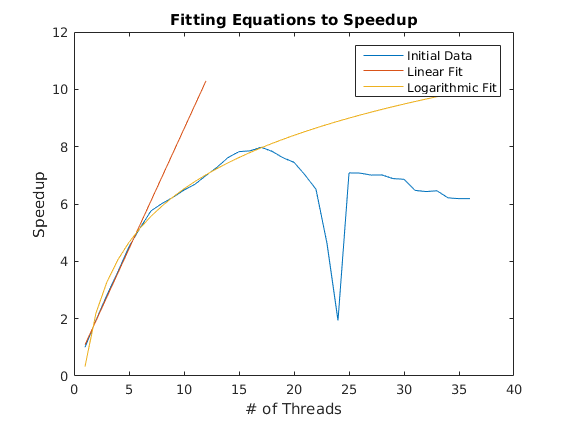
\includegraphics[width=0.6\textwidth]{../img/Debondt_fitting_v1-5crit_runtimepop.png}
\caption{Fitting equations to speedup (Debondt - EIL51 - v1-5crit - runtime scheduling).}
\label{fig:linefits}
\end{figure}




\newpage
\section{Discussion} \label{sec:discussion}
Many of the characterizations of the evolutionary strategy can be seen in Section \ref{sec:implementation}. To summarize the section, the speedup was mostly dependent on the population size and the resultant fitness was mostly dependent on the number of iterations. A suitable relationship between optimal runtime, fitness value, and speedup was found to be a population of 500 individuals and a number of iterations around 10000. Population size had a large effect on speedup since the main parallelization is in a loop over the individuals in a population. As the number of threads and the population size converge, the speedup decreases. Dramatic decreases can be seen when the number of threads reaches roughly half of the population size. At this point, a significant number of threads are left hanging as the others perform work. 

Tour size was another parameter that greatly affected speedup. As was shown Figure \ref{fig:tours}, As the tour size increased, the speedup did as well. %TODO line fit this?
This behaviour seemed to be logarithmic with the number of cities in the tour. The speedup dropped off below about 75 cities, and seemed to reach a peak around 1000 cities. This is because the most computationally rigorous section of the code is the fitness evaluation. The fitness evaluation calculates the overall distance travelled in a tour via the euclidean distance formula. Since any tour traverses each city, the number of computations required by the fitness evaluation will depend on the number of cities. During the fitness evaluation, each thread is doing useful work. If the tour size is small, then the threads may spend more time looping over the shared index variables. The proportion of useful work is therefore greater when the city size is greater.

As can be seen in many of the tests, the speedup on Debondt dropped off rapidly at around 24 threads. As was discussed previously, the Debondt system has 24 threads (virtual cores) and 12 physical cores. As with the Lenovo system, the number of virtual cores is due to hyperthreading. Hyperthreading takes advantage of the architecture of the CPU. Since CPUs typically have different components for floating point calculations, integer calculations, and I/O, different threads can theoretically be using the different sections of the CPU at the same time. This doesn't create extra physical cores, but it typically speeds up performance by 10-30\%. Although hyperthreading is typically good for everyday computing, it may cause issues in certain parallel and high performance computing applications. This is due to increased memory contention, cache misses, and other performance bottlenecks. Since hyperthreading does not create extra cores, you really only have full support for 12 threads, but speedup over 12 threads can be, and is, achieved \cite{leng2002study}.

The severe drop-off at 24 threads is likely due to other processes on the system combining poorly with the hyperthread scheduling. When there are fewer than 20 or so threads, there is enough processing power for both the program and the other system processes. As the number of processes approaches 24, it is more likely that the thread will be started on an occupied core. OpenMP attempts to migrate these threads to optimize runtime through their thread migration and CPU affinity settings. If OpenMP migrates the thread to a different physical processor, there could be cache coherency issues though. Alternatively, if there isn't migration, the thread could be locked to a virtual core. Since this core is only virtual, the other occupying thread could be pushing the physical core to 100\% usage, leaving the thread waiting. 

As is shown in Figure \ref{fig:tours}, which shows the speedup over different tour lengths, longer tours do not suffer as much of a performance hit. This points to thread migration as the likely culprit. Longer tours are more likely to remain on a core through the duration of their work. It would only be during the iteration, when the thread is doing comparatively less work, that it will be migrated. Therefore, shorter tours, which iterate more quickly, will tend to be migrated more often. 

On the same figure, it is shown that when the thread count exceeds the number of cores, the speedup levels out. In this case, thread migration is more likely to occur. This would point to thread binding as the more likely culprit, which is counter to the earlier point. It may be that there is a combination of the two at play. When the number of threads is slightly less than the number of virtual cores, thread migration occurs. This migration will move the threads to other cores, but the move is suboptimal since almost all of the cores are in use. When there are more threads than cores, thread migration also occurs, but each move is essentially equivalent since all the processors will have nearly the same amount of work on them. So, although the threads migrate, the migrations are less likely to cause issues. This is speculative though. Further testing would involve turning off hyperthreading in addition to changing more of the environment variables, such as \texttt{OMP\_PROC\_BIND} and \texttt{GOMP\_CPU\_Affinity}. 
%TODO this would probably be better shown on a graph where the negative speedup is on the same scale of magnitude


\newpage
\section{Conclusions}
Unfortunately, I was unable to implement everything I had planned for this project. The testing phase took up a considerable portion of the overall project time. Each test took anywhere between thirty minutes and several hours to complete. Although running each test didn't take too much effort, it was still a bottleneck in the development process. To assuage this, I parallelized my workflow by offloading the testing to the Debondt server. This meant that I could develop new code and test small instances locally while running full characterizing tests on previous versions remotely. Whenever a suitable update was created, I would offload it to the server. This isn't ideal because I wouldn't fully know the characteristics of the new version until much later, but it did allow for quicker release and versioning. The main issue with testing on the server was that I didn't know who else was using it. Although I believe that I had most of the Debondt's resources, there is a chance that other programs were running during certain tests. This would certainly skew the results.

In running the tests, I attempted some formalization by running the majority of the simulations with the same parameter values and data sets. In hindsight, it would have been good to develop a more formal testing framework though. As it was, I simply would update the parameters, run the system, then paste the output into a \texttt{.dat} file. Although this worked, it wasn't the most convenient. If I had pushed the output directly to files this would have been quicker. Changing these values for testing wasn't the most intuitive in my system though. With a formalized testing framework I would have been able to vary my tests with greater ease. Developing such a system probably would have taken more time than it was worth, but planning out the testing process more thoroughly could have saved time. 

Saving the output, then running analysis on the data later was certainly a good idea. Initially I planned on graphing the results immediately. It was only my limited knowledge of C++ that guided me towards matlab. Thankfully though, performing the analysis in this manner meant that I had more control over the graphing process. If the system had output a graph directly without saving the data, I would not have been able to evaluate as many, or as complicated, comparisons. Only by running analysis in this manner was I able to provide the best data visualizations and comparisons through the fewest number of test iterations.

If I had more time I would do the following:
\begin{itemize}
\item A suitable crossover implementation and a more variable selection method: Currently the framework lacks a crossover algorithm. As such, it is not a true genetic algorithm. Also, the parent selection is takes place between the initial individual and its mutated offspring, so it is hard to extend to different selection types. The trouble is in extending the population out of the single iterative loop. I have had trouble in maintaining speedup when trying to create create a crossover. The trouble mainly lies in the vector data type. Since this was my first C++ program, I didn't have enough knowledge of proper construction and data management. I thought that vectors would be a good way to store the data, but now I am unsure. Since the population and individual sizes were known beforehand, it might have been easier to simply use an integer array.
\item A visualization for the TSP solution: Initially I had planned on creating a sort of bitmap or heatmap to visually display the individual for intra and inter population comparisons. The plan was to ascribe each index of a matrix to a city in the tour. This index-city pairing would be immutable for the specific tour being run. The value at the index could then be one of several analysis, including the distance from the city at the index to the next city in the tour; the location of the city in the tour; or the distance of that city to a fixed point. There are a great number of ways to generate this visualization, as long as the cities at each index in the matrix are the same across individuals, the visualization should provide a good comparison.
\item Make the framework more extensible: Currently the system is only tailored towards the travelling salesperson algorithm, and it is rather constrained insofar as that. Ideally, the bulk of the framework would be general evolutionary operators and the bulk of the runtime logic for the evolutionary process. The individual's construction and fitness evaluation could be moved to a separate file. Since only really the individual and the fitness evaluation are implementation specific, the user would only have to alter this file to change the algorithm being evolved.
\item Better organization of the code base: Currently, the framework exists as a single file. Moving the evolutionary operators to a separate file would greatly increase readability.
\item Further testing with thread migration, processor binding, and hyperthreading as discussed in Section \ref{sec:discussion}.
\end{itemize}

\newpage
In summary, the initial proposal was too large a task for one single person to take within the timeframe of this project. Perhaps if I had several people, then I could have realized my initial plans more fully. Initially, this project was geared towards creating a parallelized framework to view divergent evolutionary behaviour. As development progressed however, the focus shifted more towards optimizing the parallelism. Although the current version is lacking in features, it is likely to have far greater speedup than the original plans would have allowed for. Perhaps the remainder of this framework can be a future project of mine.


%\subsection{Simple Sequential}
%\subsubsection{Population Based}
%\begin{tabular}{ c | c | c | c | c }
% 1 & 100 & 100 & 1006.61 & 0.0594495 \\
% 1 & 200 & 100 & 971.531 & 0.116636 \\
% 1 & 300 & 100 & 983.57 & 0.179451 \\
% 1 & 400 & 100 & 940.753 & 0.23334 \\
% 1 & 500 & 100 & 985.453 & 0.292069 \\
% 1 & 600 & 100 & 995.133 & 0.353345 \\
% 1 & 700 & 100 & 976.031 & 0.438044 \\
% 1 & 800 & 100 & 959.766 & 0.466137 \\  
% 1 & 900 & 100 & 969.391 & 0.522619 \\
% 1 & 1000 & 100 & 972.207 & 0.585324 \\
% 1 & 2000 & 100 & 942.047 & 1.17845  \\
% 1 & 3000 & 100 & 938.467 & 1.88575 \\
% 1 & 4000 & 100 & 940.066 & 2.37096 \\
% 1 & 5000 & 100 & 927.209 & 3.02321 \\
% 1 & 6000 & 100 & 920.407 & 3.73201 \\
% 1 & 7000 & 100 & 919.812 & 4.54565 \\
% 1 & 8000 & 100 & 922.916 & 5.10203 \\
% 1 & 9000 & 100 & 929.764 & 5.55095 \\
% 1 & 10000 & 100 & 925.476 & 6.07093 \\
%\end{tabular}

%\subsubsection{Iteration Based}
%\begin{tabular}{ c | c | c | c | c }
% 1 & 100 & 100 & 1005.18 & 0.0612377 \\
% 1 & 100 & 200 & 879.523 & 0.117883 \\
% 1 & 100 & 300 & 800.886 & 0.174866 \\
% 1 & 100 & 400 & 791.031 & 0.237152 \\
% 1 & 100 & 500 & 716.329 & 0.292422 \\
% 1 & 100 & 600 & 700.984 & 0.351435 \\
% 1 & 100 & 700 & 698.819 & 0.41049 \\
% 1 & 100 & 800 & 685.63 & 0.476722 \\
% 1 & 100 & 900 & 667.82 & 0.530665 \\
% 1 & 100 & 1000 & 650.368 & 0.59416 \\
% 1 & 100 & 2000 & 573.286 & 1.23812 \\
% 1 & 100 & 3000 & 534.997 & 1.79002 \\
% 1 & 100 & 4000 & 521.264 & 2.36564 \\
% 1 & 100 & 5000 & 510.855 & 2.95029 \\
% 1 & 100 & 6000 & 503.941 & 3.781 \\
% 1 & 100 & 7000 & 505.155 & 4.3372 \\
% 1 & 100 & 8000 & 498.558 & 4.94316 \\
% 1 & 100 & 9000 & 502.808 & 5.59283 \\
% 1 & 100 & 10000 & 497.015 & 6.0404 \\
%\end{tabular}

%\subsubsection{Thread Based}
%\begin{tabular}{ c | c | c | c | c }
%1 & 500 & 10000 & 480.492 & 28.9301 \\
%2 & 500 & 10000 & 481.042 & 17.08 \\
%3 & 500 & 10000 & 486.164 & 19.4246 \\
%4 & 500 & 10000 & 481.419 & 16.1616 \\
%6 & 500 & 10000 & 478.596 & 18.4624 \\
%8 & 500 & 10000 & 484.597 & 18.7737 \\
%16 & 500 & 10000 & 484.133 & 19.2235 \\
%32 & 500 & 10000 & 485.378 & 20.5241 \\
%64 & 500 & 10000 & 480.417 & 20.9859 \\
%\end{tabular}



{\small
\bibliographystyle{ieee}
\bibliography{egbib}
}


\end{document}